\section{Discussion}
We claim that our implementation is correct-by-construction because it is obviously correct because the code \textit{is} the model specification - we have closed the gap between the specification and its implementation. Still we need to verify the dynamics and test the system for its numerical behaviour under varying $\Delta t$.

\begin{figure}
	\centering
	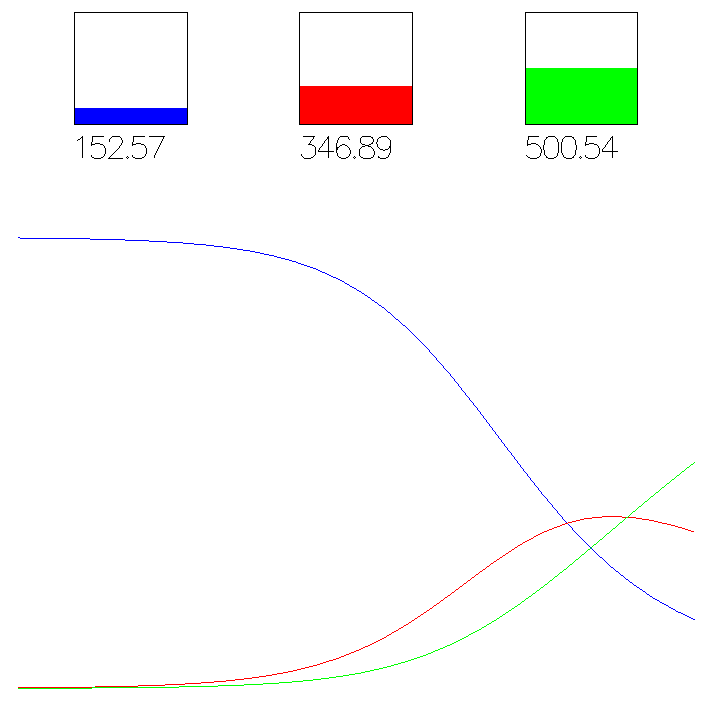
\includegraphics[width=.4\textwidth, angle=0]{./fig/visualisation_t50.png}
	\caption{Snapshot of a real-time visualisation of a SIR compartment model simulating using Haskell. Population Size $N$ = 1,000, contact rate $\beta =  \frac{1}{5}$, infection probability $\gamma = 0.05$, illness duration $\delta = 15$ with initially 1 infected agent. Simulation run until $t = 50$.}
	\label{fig:sir_sd_dynamics}
\end{figure}

TODO: argue why it is correct-by-construction, why reproducible guaranteed at compile-time,... support our initial hypothesis and claims from introduction

TODO: integral is the fundamental function
- need to show that it indeed implements the rectangle rule. 
- show that with too large dt we arrive at slightly different results after same time-steps
- implement a better integral function using better behaved numerical integration